\documentclass[UTF8]{article}
\usepackage{ctex}
\usepackage{ulem}
\usepackage{dsfont}
\usepackage{amssymb}
\usepackage{amsmath}
\usepackage{graphicx}
\newtheorem{thm}{定义}[section]
\newtheorem{notation}[thm]{记号}
\newtheorem{lemma}[thm]{引理}

\makeatletter
\newcommand{\rmnum}[1]{\romannumeral #1}
\newcommand{\Rmnum}[1]{\expandafter\@slowromancap\romannumeral #1@}
\makeatother
\newcommand{\dperp}{\perp\!\!\!\perp}

\title{13 集合与子集\\Sets and subsets\\[2ex]\begin{large}读书笔记\end{large}}
\author{许博}
\date{}

\begin{document}
\maketitle
	\section{在$\lambda{\rm D}$中处理子集}
	\noindent
	之前我们已经在类型理论中,将类型解释为集合,但当考虑到子集时,会有诸多问题需要考虑。比如类型的唯一性与对子集的自然观点矛盾,假设$S$是一个集合而$T$是$S$的真子集,令$c\in S$,则应有$c\in T$,也即$c:S\Rightarrow c:T$,显然违背了类型唯一性。
		
		另一个例子是,令$P$是$S$中的元素的一个属性,集合$\{x\in S|Px\}$表示$S$中满足$P$的所有元素,则对于$c:S$,$c:\{x\in S|Px\}$是不可判定的,因为在类型理论中,类型检查需要是可判定的,即给定的合法的项,一定能够得它的类型匹配与否,而非尚未知晓的答案,且判定任意命题可证明是不可判定的。
		
		类型的可判定性使得类型理论称为用于证明检查与查找的一个强大系统,另一方面,阻止了对于子集的一般处理方式。而类型理论的可判定性以及类型的唯一性需要得到保留,以使我们的推导系统保持作为证明检查基础的有效性。因此,我们决定保留类型理论的可判定性,以及接受这个选择所带来的所有后果,尤其是关于子集的。
		
		在描述子集的表示方式之前,首先介绍数学中与集合有关的一些概念。
		
		$x\in S$表示$x$是$S$的一个成员。$S$是$T$一个子集,如果$S$的所有成员都是$T$的成员。除此之外还有集合的相等性,并集,交集,差集,补集,幂集以及笛卡尔积等概念,可自行查阅。
		
		在类型理论$\lambda{\rm D}$中,我们通过一种顺理成章又精彩的方式表示子集:使用谓词。假设存在一个集合$S$,集合$V$是$S$中满足谓词$P$的元素的集合,也即$V\subset S$,显然对于任意的$x:S$,都有$x\in V\Leftrightarrow P(x)$。此时,我们使用谓词$P$来表示子集$V$,此时对于$S$的子集$V$而言,$V$是在$S$上的谓词。如果$x\in V$,则$Vx$成立。子集的表示如下:\\
		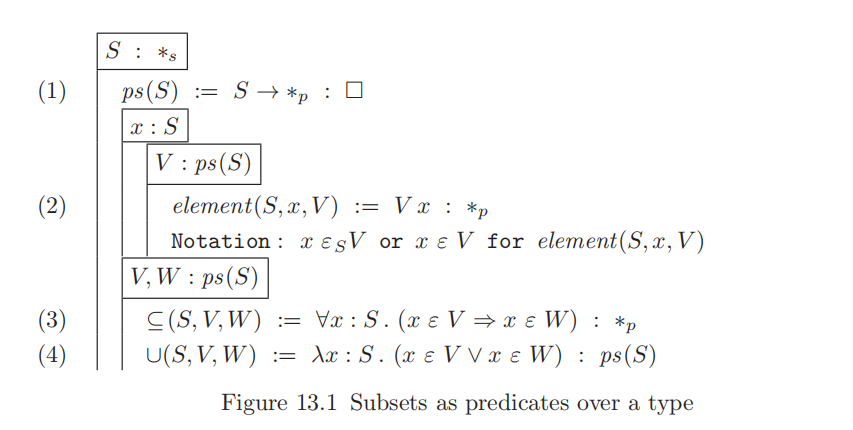
\includegraphics[width=0.93\linewidth]{"../imgs/13-1.png"}
		
		其中,$ps(S)$表示$\mathcal{P}(S)$,也即集合$S$的幂集,可见$ps(S)$的成员均是$S$的子集,也即在$S$上的谓词。同时还定义了关系$\subseteq$和$\cup$。
\end{document}
